% Preamble
\documentclass[11pt]{article}

% Packages
\usepackage{a4wide}
\usepackage{graphicx}
\usepackage{url}
\usepackage[nottoc]{tocbibind}
\usepackage{listings}
\usepackage{caption}
\usepackage{amsmath}

% Author
\author{Van Dam, Thijs\\
\and
Bos, Sander\\
}
\title{\huge The Animal Kingdom}
\date{April 2018}

\setlength{\parindent}{0em}
\setlength{\parskip}{1em}

\DeclareCaptionFormat{cancaption}{#1#2#3\par}
\DeclareCaptionLabelFormat{cancaptionlabel}{#1}
\captionsetup[figure][number]{format=cancaption,labelformat=cancaptionlabel}
\graphicspath{{images/}}


% Document

\begin{document}
    \maketitle
    \thispagestyle{empty}
    \newpage
    \newpage
    \setcounter{page}{1}
    \section{Introduction}\label{sec:introduction}
    In this document we discuss the following topics:
    \begin{itemize}
        \item Steering
        \item Path planning
        \item Behaviour
        \item Fuzzy logic
    \end{itemize}
    
    To understand the context of this game, we will first give a short explanation of the game/simulation itself.
    
    \subsection*{About the game}\label{subsec:about}
    Somewhere in Africa, a herd of gazelles is gathering food.
    At the same time a pride of lions is getting quite hungry and thus sees the gazelles as a tasteful meal.
    The gazelles notice the lions are getting closer and closer.
    They start to run.
    It becomes a race of life and death\ldots
    
    \subsection*{Notes}\label{subsec:notes}
    All diagrams and images are also available as seperate image.

    \newpage
    %-----------------------------------------------------------------------------------------
    \tableofcontents
    
    \newpage
    %-----------------------------------------------------------------------------------------
    \section{Steering}\label{sec:steering}
    We implemented all the simple steering behaviours that were provided.
These are \textbf{seek}, \textbf{flee}, \textbf{arrive} and \textbf{wander}.
Last but not least we implemented two advanced steering behaviour: \textbf{obstacle avoidance} and \textbf{explore}.
Firstly, we will discuss every behaviour we implemented a little.
\subsection[Describing the steering behaviours]{Behaviours}\label{subsec:behaviours}
In this section I will talk about every behaviour slightly.
We will discuss our way of implementing each behaviour and how it works.
\subsubsection{Seek}
This was the first behaviour we implemented, simply because we thought this was the easiest behaviour to implement.
We couldn't have been more right.
The seek algorithm simply moves towards a goal at max speed, and will still be moving at max speed when arriving at the target.
Since it doesn't slow down, it just passes the goal, and then turns around to, again, reach towards this goal at max speed.
This results in moving bach and forth, through the goal.
\paragraph{Implementation}
Thus, the algorithm needs a goal (\textit{BaseGameEntity}), and a user, which we called movingEntity (\textit{MovingEntity}).
Having this goal, we could determine which direction the movingEntity should go to, in order to reach this goal.
Now, we can return a force (\textit{Vector2D}), equal to the max possible force for the current movingEntity.
To finish his behaviour, only the velocity our movingEntity currently has, has to be substracted from this force.
This way our entity won't make a sharp, but a smooth turn.
\subsubsection{Flee}
The flee behaviour is not much more than the seeking behaviour, but reversed.
With this I mean that in stead of moving towards a target at max speed, the entity moves away from a target at max speed.
One addition is that when there is an obstacle in between the target and our entity, the algorithm should just do nothing.
\paragraph{Implementation}
First, we check if in between the entity and the goal is an obstacle present, if there is: do nothing!
If there isn't, go on with your calculation.
The calculation of the fleeing behaviour is almost exactly the same as the calculation of the seek behaviour.
Only, when you have found the direction you want to go in, you turn it around.
This is simply done by creating a new desired velocity, called newDesiredVelocity (\textit{Vector2D}), and inverting the X and the Y of the already found velocity.
\subsubsection{Arrive}
This is also a behaviour that is much like seek.
The difference is that, where seek continues to move with max speed at the target, the arrive behaviour will slow down till it reaches its target.
\paragraph{Implementation}
Actually, the implementation of the arrive behaviour is a lot different from seek.
Arrive also has to take the deceleration speed into account, and the distance between the moving entity and the target.
We have put a boundry on calculate this on a distance of 0.05, because everything after that will be unseeable movements and really specific calculations.
This is not needed.
The closer the entity is to the target, the slower it will be.
We achieve this by dividing the speed by the distance and multiplying that with the distance to our target, getting a desiredVelocity (\textit{Vector2D}).
Lastly, we have to substract the current velocity from the currentVelocity again.
\subsubsection{Wander}
Then, finally, we come across a more interesting behaviour, making it seem like the entity is wandering over the screen.
This wandering should happen as random as it could, and will be used when the entities have nothing much to do.
This way to do this is to get a \textbf{circle} at a certain distance in front of our entity, in the direction of our entity as well.
On this circle, choose a \textbf{point} to move towards, and make this point move along the circle in a random direction. (up and down)
\begin{figure}[h!]
    \begin{center}
        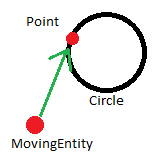
\includegraphics[width=10em]{WanderBehaviour.png}
    \end{center}
    \caption{Wander behaviour explanation example}
    \label{fig:WanderBehaviourExplanation}
\end{figure}
\paragraph{Implementation}
Looking at the image, it looks like a pain to implement, but it actually is quite easy!
To do it we actually need some extra variables, namely:
\begin{itemize}
    \item Circle distance
    \\\textit{The distance between the MovingEntity and the middle of the circle.}
    \item Circle radius
    \\\textit{The radius of the circle.}
    \item Turning angle
    \\\textit{The angle the point has to 'turn' when this value is calculated.}
    \item Previous angle
    \\\textit{To remember the previous of the dot (so we can move it from that point), we just remember the last angle inside a variable!}
\end{itemize}
First, you calculate the direction the entity currently goes to.
Somewhere inbetween you can change the angle to a new angle.
Since this should happen randomly, add or substract (chosen randomly) the turning angle from/to the previous angle.
Determine the middle of the circle and calculate the angle of where the piont should be.
Now just return the vector towards that point and you're done.
\subsubsection{Obstacle avoidance}\label{sec:ObstacleAvoidance}
All in all we spent the most time finding a solution to obstacle avoidance.
We will only explain how this behaviour works, and in a later part of this document we will talk about our problem.
A rectangle gets drawn in front of the movingEntity in the direction the entity goes to.
Within this rectangle, collisions with obstacles get checked.
If there is a collision with an obstacle, create a force in the opposite direction.
\begin{figure}[h!]
    \begin{center}
        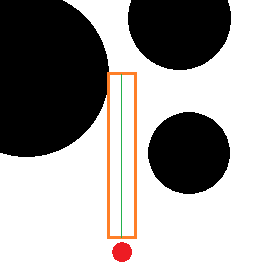
\includegraphics[width=10em]{ObstacleAvoidance.png}
    \end{center}
    \caption{Obstacle avoidance example}
    \label{fig:ObstacleAvoidanceExplanation}
\end{figure}
\paragraph{Implementation}
Compared to the explanation, the implementation is fairly complex.
This is because, when you have a lot of obstacles, it is really ineffici\"ent to check your collision with all the obstacles.
So, we filter the obstacles on being within the range of movingEntities current velocity in a list, \textit{obstaclesWithinRange}.
The rectangle drawn in front of our entity, only is as big as your own velocity, making it impossible to even reach obstacles that are further away than your velocity.
To see where each obstacle is compared to our entity, we translate these obstacles to our 'local space'.
This means nothing more than 'position compared to our entity its position'.
Do this by translating all obstacles in \textit{obstaclesWithingRange} with position of our current entity.
After you have translated these obstacles, rotate them according to the direction of our current moving entity.
If you have done this, all obstacles with a negative X value will be 'behind you'. (since, for the axial system, you rotated them relative to the right of our current entity)
For each obstacle in front of you and within your range, check if this obstacle is inside our rectangle.
If the obstacle collides with our rectangle, generate a force in the opposite direction of the obstacle relative to our rectangle.
\subsubsection{Explore}
%TODO: finish
\subsection[Problems we had during implementing these behaviours]{Problems}\label{subsec:problems}
There were some major problems we came across during the implementation of some behaviours.
Though, all in all, we didn't have that many and we got the behaviours working pretty fast.
Some minor mistakes we made were mixing up a vector for indication a position, and for indicating a direction and speed.
Since both are just \textit{Vector2D}'s, this could be confusing.
This wasn't much of a hassle to fix and mixing these up only resulted in some strange outcomes, which actually cost some time.
The one major problem we had was with (\ref{sec:ObstacleAvoidance}) Obstacle voidance.
On calculating the local space of an object, we had an issue rotating it.
We only found a way to calculate the angle to rotate with, with \textit{Math.Atan(X/Y)}.
The problem with this is that it it returns the exact same value with both the X and Y negative, as with both the X and Y positive.
This is also the case with a negative X and a positive Y, as with a positive X and a negative Y.
Now, resulting our obstacles to be rotated by the same value if its in front of our entity, as when it's behind our entity.
Messing around with this, we couldn't come up with a good, clean solution to fix this.
After a while, we found the \textit{Math.Atan2(double input)} function, which actually returns different values for the edgecases as described before.
Our big solution to this problem!
\subsection[How the steering behaviours are combined]{Combining behaviours}\label{subsec:combiningBehaviours}
A manager (\textit{SteeringBehaviours})is used per MovingEntity to manage all the the different possible behaviours.
For each implemented behaviour, properties exist in the SteeringBehaviours class.
If a behaviour is turned on for a certain entity, an instance will be created under that certain name.
A behaviour can be turned on by calling the \textit{[BehaviourName]On(required params)};, and it can be turned off by calling \textit{[BehaviourName]Off()};
In this manager there are two methods that handle all the actions for the behaviours.
There is the \textit{Calculate()}-method, calling all the calculates for the different, instantiated behaviours.
It creates a vector (\textit{Vector2D}) and adds all the forces gained by the behaviours up, and finally truncates it with the max force (\textit{MovingEntity.DMaxForce}) of the current entity.
Then, there is the \textit{DrawBehaviours()}-method, doing exactly as it says.
Inside each behaviour we inserted a \textit{DrawBehaviours()}-method as well, to give a visual representation of the forces and methods working for this behaviour.
\subsection[The class diagram of our behaviour system]{Class diagram}
\begin{figure}[h!]
    \begin{center}
        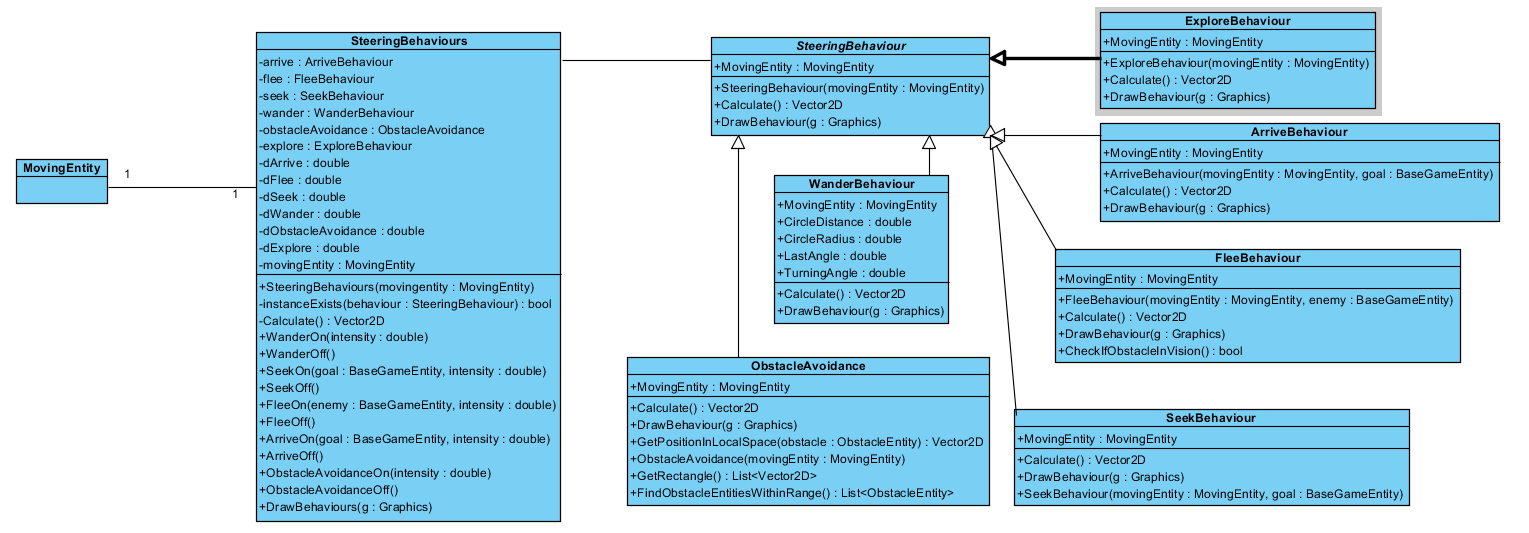
\includegraphics[width=35em]{BehavioursClassDiagram.PNG}
    \end{center}
    \caption{Steering behaviours class diagram}
    \label{fig:SteeringBehavioursClassDiagram}
\end{figure}
\newpage
%-----------------------------------------------------------------------------------------

    \newpage
    %-----------------------------------------------------------------------------------------
    \section{Path planning}\label{sec:pathPlanning}
    This section contains all information about the path planning algorithms and structure used in 'The Animal Kingdom'.
First the structure will be discussed, then we will give an illustration of how the graph is rendered and in the last part of this section,
the implementation of the used path-finding algorithms is explained.

\subsection{Structure}\label{subsec:pathstructure}
Buckland describes\cite{pgaie} a well-structured approach to splitting logic for the pathfinding.
This same structure is what we used in our application, although we have made some changes to fit our own needs.
The application contains one instance of a \textit{PathManager} and each (moving) entity contains a \textit{PathPlanner}.
The \textit{PathPlanner} is what is used to request a new search with the specified algorithm (A* or Dijkstra).
When a request is done, the \textit{PathPlanner} registers itself in the \textit{PathManager}.
Using a \textit{PathManager} makes it possible to manage and control all search requests from one place.
This is especially useful when you want to implement time-slicing or other logic that restricts the amount of search cycles per update.
The latter case is what we use it for.
\textit{PathManager} contains a function \textit{UpdateSearches()} which lets each \textit{PathPlanner} do one or more cycle depending on the maximum cycles set while instantiating the \textit{PathManager}.
What a cycle does, will be discussed in section \ref{subsec:pathalgorithms}.\par
The class diagram below (fig.\ref{fig:pathPlanClassDiagram}) shows the structure of the pathfinding logic including the \textit{PathManager} and \textit{PathPlanner}.

\begin{figure}[h!]
    \begin{center}
        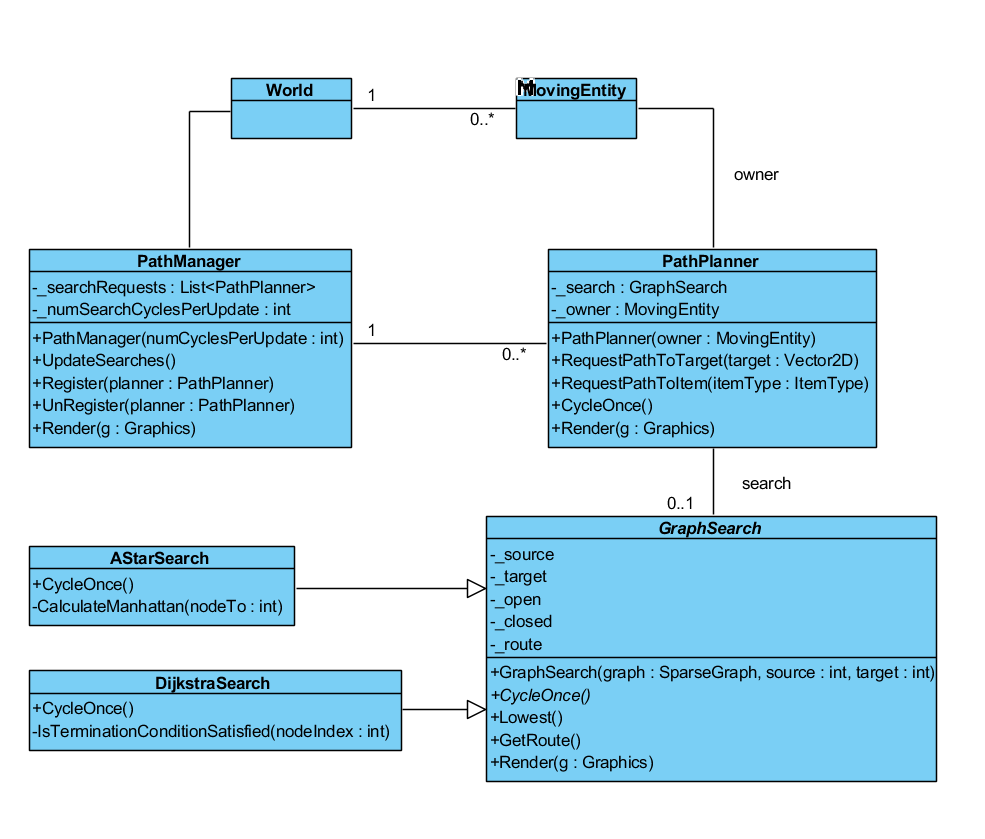
\includegraphics[width=26em]{PathFinding.png}
    \end{center}
    \caption{Path planning class diagram}
    \label{fig:pathPlanClassDiagram}
\end{figure}

\subsection{Creating a graph}\label{subsec:pathgraphcreation}
The graph in the game world is created using a floodfill.
A single point is given as its starting position and from that point edges and nodes are added in every direction.
If the placing of an edge or node is obstructed by an obstacle, it will not be created and the floodfill will continue
in the other directions.
This results in a graph that fills the complete game world.
The graph itself is not saved as a file, it is possible to do this, but because of the small area of the field,
generating a graph at the start of the application does not affect performance and loading time.
The picture below (fig.\ref{fig:pathPlanFloodfill}) demonstrates the result of using floodfill.

\begin{figure}[h!]
    \begin{center}
        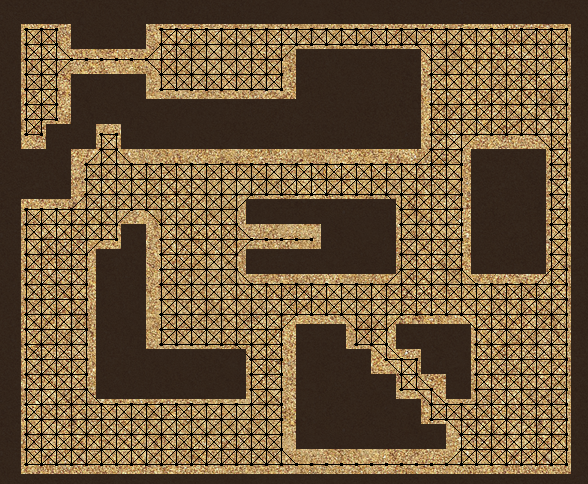
\includegraphics[width=28em]{Floodfill.png}
    \end{center}
    \caption{The result of using floodfill}
    \label{fig:pathPlanFloodfill}
\end{figure}

\subsection{Algorithms}\label{subsec:pathalgorithms}
As mentioned previously, we have implemented two path-finding algorithms in the application.
Dijkstra and A*. Each of the algorithms is implemented in a separate class extending the \textit{GraphSearch} class.
Both implementations will be discussed below.

\subsubsection{Dijkstra}\label{sec:pathDijkstra}
The first algorithm we implemented, is Dijkstra as it is also the base of the A* algorithm.
Although the algorithm was already familiar to us, implementing it was a bit more difficult than we expected.
It was not a lot of work, but it did require some thinking.
In Programming Game AI by Example, Buckland describes a version of the algorithm that looked more complex than necessary.
Luckily we found a pseudo code\cite{aapc} of A*, which by removing the heuristics, was a much better understandable version of the algorithm.\par
A first version of the algorithm was without the \textit{PathManager} and/or \textit{PathPlanner} and did not contain the \textit{CycleOnce()}.
Instead, we had a single function \textit{Search()} which did the whole search at once.
The function \textit{IsTerminationConditionSatisfied()} was added to check if an item of the specified \textit{ItemType} was found.
If a matching item was found, the algorithm was stopped and the route was returned.
The resulting route was eventually drawn on the screen by adding a \textit{Render()} function.

\subsubsection{A*}\label{sec:pathAstar}
As A* is basically Dijkstra with heuristics, it was easy to convert our existing Dijkstra algorithm to A*.
Just as with the Dijkstra algorithm, we first created a single \textit{Search()} which did the whole search at once.
The heuristic used for our implementation is Manhattan, which we calculated in \textit{CalculateManhattan()}.
The distance between all nodes is the same in the graph and each edge has a cost of 1.
Calculating the Manhattan distance was very easy as we could just calculate the distance between the current node and target location
and devide it by the length of one edge to get the estimated distance (fig.\ref{fig:pathPlanCalcManhattan}).

\begin{figure}[h!]
    \[ $$Dist_M = \dfrac{|targetLocation.X - currentLocation.X| + |targetLocation.Y - currentLocation.Y|}{15}\]
    \caption{Calculating the Manhattan distance}
    \label{fig:pathPlanCalcManhattan}
\end{figure}

\subsection{Performance}\label{subsec:pathperformance}
Because of the implementation of the \textit{PathManager} and \textit{PathPlanner} resources will be shared equally between all moving entities.
There is also a predifined maximum amount of calculation cycles per update, which prefents the game from slowing down.
At first we struggled with this, as it seemed to take much longer to find a path than previoulsy with just the single \textit{Search()} function.
After a bit of tweaking (changing the maximum amount of cycles per update) and removing a lot of \lstinline[columns=fixed]{Console.WriteLine(...)}
lines used for debugging which were clearly slowing down the calculations as they were limited by the speed of the console.\par
However, performance can still be improved.
Storing precalculated costs, or some shortest paths could dramatically improve the performance when the amount of agents increases.

    \newpage
    %-----------------------------------------------------------------------------------------
    \section{Behaviours (Goals)}\label{sec:behaviour}
    Behaviour of all entities within the game are discussed in this section.

\subsection{Structure}\label{subsec:behaviourStructure}
We have chosen to use goal-driven behaviour in our game.
Three main classes make up most of the structure, they are: \textit{Goal}, \textit{CompositeGoal} and \textit{AtomicGoal}.
As seen in the naming, a composite design pattern has been used to enable the grouping of goals while keeping the same functionalities.
This means that an \textit{AtomicGoal} can be used in the same way as a \textit{CompositeGoal} with the exception of \textit{AddSubGoal()},
which is only implemented in the composite.
This structure is used to create all strategy-level goals.

The class diagram below shows the structure (fig.\ref{fig:behaviourClassDiagram}).

\begin{figure}[h!]
    \begin{center}
        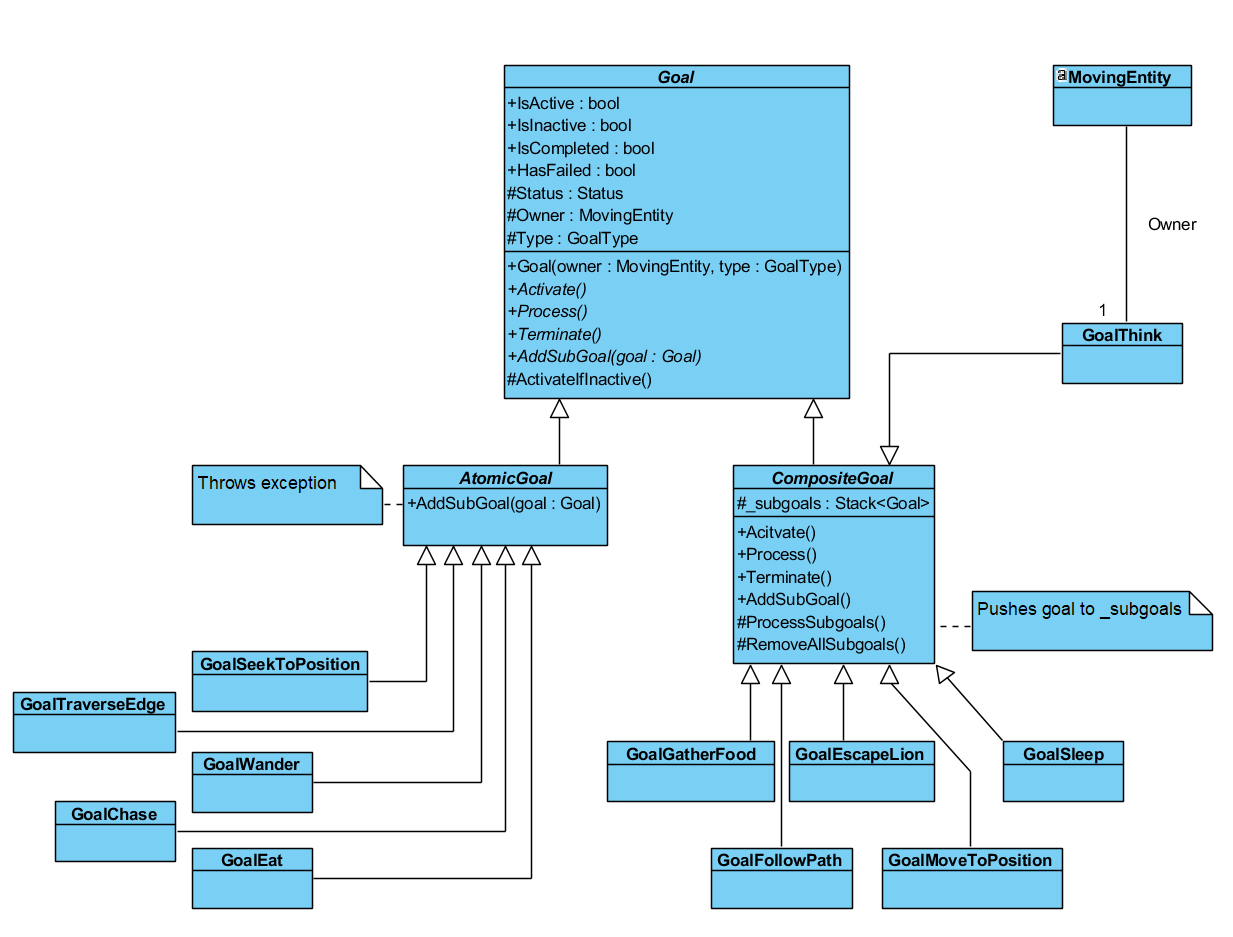
\includegraphics[width=40em]{Goals.png}
    \end{center}
    \caption{Goals class diagram}
    \label{fig:behaviourClassDiagram}
\end{figure}


\subsection{Goals}\label{subsec:behaviourGoals}
To give each entity a specific behaviour, we have created a couple of (composite) goals with some underlying atomic goals.
These goals wil be discussed below.

\subsubsection{Gather Food}\label{sec:behaviourFood}
Both the gazelles and the lions will have to gather food if they want to survive.
For gazelles it will mean that they have to find (\textit{GoalMoveToPosition}) grass or water and start eating.
Lions do not like grass, so they will have to chase (\textit{GoalChase}) a gazelle and eat it.
The gazelle will then try to escape (\textit{GoalEscapeLion}) which we will discuss in the next part.
If a lion caught a gazelle, the lion will eat (\textit{GoalEat}) the poor animal.

This is the most complex behaviour.
The \textit{GoalMoveToPosition} has as its first subgoal \textit{GoalSeekToPosition}.
This will continue until the path has been found and then \textit{GoalFollowPath} will be added with the found path.
While there is a path to follow, the \textit{GoalTraverseEdge} will be added, each time with a next node as position to travel to.
This enables the \textit{SeekBehaviour} to the given point.
If it is the last node, the \textit{GoalTraverseEdge} will start the \textit{ArriveBehaviour} to the final destination.

\subsubsection{Escape From Lion}\label{sec:behaviourEscape}
A gazelle does not want to be eaten by a lion, so it will try to escape a lion once it is within a certain range.
The \textit{FleeBehaviour} will be enabled for the gazelle, but its energy will drain.
%ToDo: Do we want flee or not, what should we do with this goal?

\subsubsection{Sleep}\label{sec:behaviourSleep}
Lions are actually lazy animals.
Once they had a nice meal, they want to sleep.
Gazelles will be very happy once that happens and they can relax for a while.
They will probably start grazing again as that is what they do most of the time.
If a lion sleeps, it won't do anything for a while, until he is fully back to strength.

This is a pretty simple goal, but very important for the lions.
It will temporarily disable all steering behaviour for the lion entity.


    
    \newpage
    %-----------------------------------------------------------------------------------------
    \section{Fuzzy logic}\label{sec:fuzzyLogic}
    \subsection{FLV Graphs}\label{subsec:flvGraphs}
The beneath diagram shows the 4 fuzzy linguistic variables for a gazelle.
These follow the rules of the next subsection.
As you can see, there is two factors a gazelle can use in order to determine if it wants to run or it wants to eat.
We also implemented fuzzy logic for the lion, but we will not describe it in this document.
\begin{figure}[ht]
    \begin{center}
        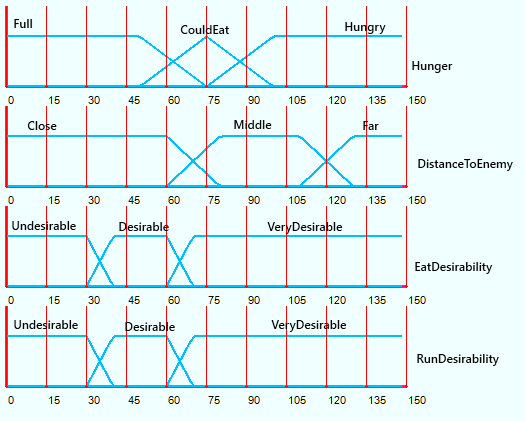
\includegraphics[width=25em]{FuzzyLogic.PNG}
    \end{center}
    \caption{Fuzzy logic explanation}
    \label{fig:FuzzyLogicExplanation}
\end{figure}
\subsection{Rulesets}
These are the rulesets used in our program.
They only portray the two decisions of a gazelle, namely wanna eat and wanna run.
The horizontal values (close, middle and far) are aimed at the distance between the gazelle and a lion.
The vertical values (full, couldeat and hungry) are aimed at the hunger the gazelle experiences.
Based on these values, the gazelle should be able to choose if gathering food is undesirable, desirable or verydesirable.
\begin{table}[ht]
    \centering
    \label{EatDesirability}
    \begin{tabular}{|l|l|l|l|}
        \hline
        & \textbf{Close}       & \textbf{Middle}        & \textbf{Far}           \\ \hline
        \textbf{Full}     & Undesirable & Undesirable   & Undesirable   \\ \hline
        \textbf{CouldEat} & Undesirable & Desirable     & Desirable     \\ \hline
        \textbf{Hungry}   & Undesirable & VeryDesirable & VeryDesirable \\ \hline
    \end{tabular}
    \caption{GazelleWannaEat}
\end{table}
\begin{table}[ht]
    \centering
    \label{|RunDesirability}
    \begin{tabular}{|l|l|l|l|}
        \hline
        & \textbf{Close}       & \textbf{Middle}        & \textbf{Far}           \\ \hline
        \textbf{Full}     & VeryDesirable & Desirable       & Undesirable     \\ \hline
        \textbf{CouldEat} & VeryDesirable & Undesirable     & Undesirable \\ \hline
        \textbf{Hungry}   & VeryDesirable & Undesirable     & Undesirable \\ \hline
    \end{tabular}
    \caption{GazelleWannaRun}
\end{table}
\subsection{Calculation}\label{subsec:calculation}
In this section I will do two calculations, to show how the fuzzy logic works, and how it works with our implementation.
For the first situation we pick two variables for the antecedents, namely 140 for the DistanceToEnemy and 80 for the Hunger.
\begin{figure}[ht]
    \begin{center}
        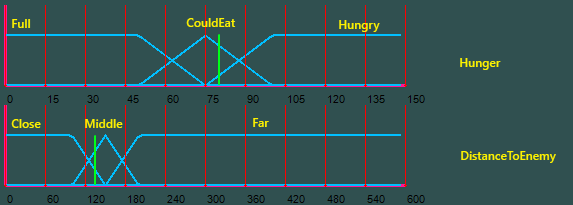
\includegraphics[width=20em]{FuzzyLogicCaseOne.PNG}
    \end{center}
    \caption{Fuzzy logic case 1}
    \label{fig:FuzzyLogicCaseOne}
\end{figure}
As you see, we drew a line on the value of 80 in the Hunger FLV, and a line on the value of 140 on the DistanceToEnemy FLV\@.

Right now, we can determine that for the first flv:

\begin{equation}
    Hunger_{Full}(80) = 0
\end{equation}

\begin{equation}
                  Hunger_{CouldEat}(80) = 0.8
\end{equation}

\begin{equation}
                  Hunger_{Hungry}(80) = 0.2
\end{equation}


And for the second FLV:

\begin{equation}
    DistanceToEnemy_{Close}(140) = 0
\end{equation}
\begin{equation}
    DistanceToEnemy_{Middle}(140) = 0
\end{equation}
\begin{equation}
    DistanceToEnemy_{Far}(140) = 1
\end{equation}

Now, for both consequents we can fill in the table.
\begin{table}[ht]
    \centering
    \label{EatDesirabilityCaseOne}
    \begin{tabular}{|l|l|l|l|}
        \hline
                          & \textbf{Close}    & \textbf{Middle}     & \textbf{Far}           \\ \hline
        \textbf{Full}     & Undesirable (0)   & Undesirable   (0)   & Desirable     (0)   \\ \hline
        \textbf{CouldEat} & Undesirable (0)   & Desirable     (0)   & VeryDesirable (0.8) \\ \hline
        \textbf{Hungry}   & Undesirable (0)   & VeryDesirable (0)   & VeryDesirable (0.2) \\ \hline
    \end{tabular}
    \caption{EatDesirability}
\end{table}
\begin{table}[ht]
    \centering
    \label{RunDesirabilityCaseOne}
    \begin{tabular}{|l|l|l|l|}
        \hline
                          & \textbf{Close}      & \textbf{Middle}     & \textbf{Far}\\ \hline
        \textbf{Full}     & VeryDesirable (0)   & VeryDesirable (0)   & Undesirable (0)   \\ \hline
        \textbf{CouldEat} & VeryDesirable (0)   & Desirable     (0)   & Undesirable (0.8) \\ \hline
        \textbf{Hungry}   & VeryDesirable (0)   & Desirable     (0)   & Undesirable (0.2) \\ \hline
    \end{tabular}
    \caption{RunDesirability}
\end{table}
This can be calculated into a max value for all FuzzySets.
\begin{table}[ht]
    \centering
    \label{InferedConclusionsEatDesirability}
    \begin{tabular}{|l|l|}
        \hline
        \textbf{Undesirable}   & 0   \\ \hline
        \textbf{Desirable}     & 0   \\ \hline
        \textbf{VeryDesirable} & 0.8 \\ \hline
    \end{tabular}
    \caption{Infered conclusions EatDesirability}
\end{table}
\begin{table}[ht]
    \centering
    \label{InferedConclusionsRunDesirability}
    \begin{tabular}{|l|l|}
        \hline
        \textbf{Undesirable}   & 0.8   \\ \hline
        \textbf{Desirable}     & 0     \\ \hline
        \textbf{VeryDesirable} & 0     \\ \hline
    \end{tabular}
    \caption{Infered conclusions RunDesirability}
\end{table}
Now we have these infered conclusions, we can defuzzify the consequents!
We will use MaxAV, since MaxAV is mainly used in our program.
Also, centroid is implemented, but we wont discuss that in this documentation.
For this, we have to calculate the maxima of both consequent FLV's.
You can check this in the graph above, right now I just took the values we chose to draw the graphs.
In the EatDesirability consequent, the maxima are:
\begin{equation}
    Eat_{Undesirable} = \frac{0 + 30}2 = 15
\end{equation}
\begin{equation}
    Eat_{Desirable} = \frac{40 + 60}2 = 50
\end{equation}
\begin{equation}
    Eat_{VeryDesirable} = \frac{70 + 150}2 = 110
\end{equation}
And now defuzzify with MaxAV through the following formula:
\begin{equation}
    MaxAV = \frac{15 * 0 + 50 * 0 + 110 * 0.8}{0.8} = 88
\end{equation}
In the RunDesirability consequent, the maxima are:
\begin{equation}
    Run_{Undesirable} = \frac{0 + 30}2 = 15
\end{equation}
\begin{equation}
    Run_{Desirable} = \frac{40 + 60}2 = 50
\end{equation}
\begin{equation}
    Run_{VeryDesirable} = \frac{70 + 150}2 = 110
\end{equation}
And now defuzzify with MaxAV through the following formula:
\begin{equation}
    MaxAV = \frac{15 * 0.8 + 50 * 0 + 110 * 0}{0.8} = 12
\end{equation}

\newpage
\subsection{Code fragment}
These are actually not the same values as the above calculations.
This is because we changed the program later to fit our fuzzy system better, but we did not have time to change the docs.
Fuzzy logic works just fine and you can calculate it through the application.
Right now we will do the exact calculation as above, but then with our code.
First, we will create a fuzzy module with two antecedents.

\begin{figure}[ht]
    \begin{center}
        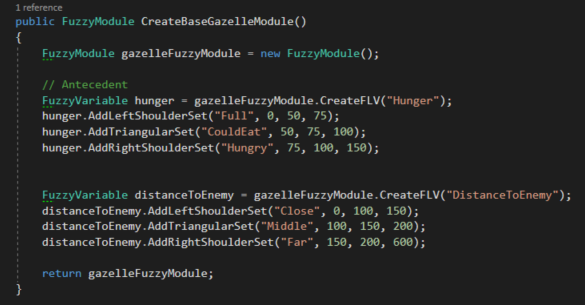
\includegraphics[width=40em]{FuzzyModuleGazelle.PNG}
    \end{center}
    \caption{Fuzzy module gazelle}
    \label{fig:FuzzyModuleGazelle}
\end{figure}
\newpage
Then, we will create two consequents with its own rulesets, namely WannaRun and WannaEat, as following!

\begin{figure}[ht]
    \begin{center}
        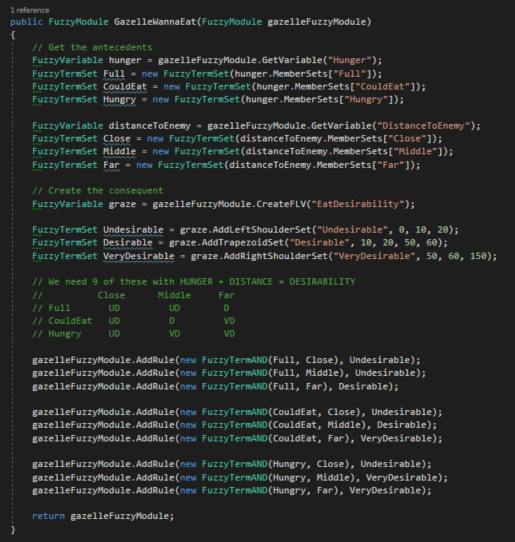
\includegraphics[width=40em]{FuzzyWannaEat.PNG}
    \end{center}
    \caption{Fuzzy wanna eat consequence + ruleset}
    \label{fig:FuzzyWannaEat}
\end{figure}
In this figure you see firstly we get all the variables from our already created module and create new TermSets so we can use them in our rules.
Next, we create a FLV according to the values of this module.
The values inside the AddLeftShoulderSet are predefined, and you can just adjust them if you want to have a different result.
Then, we add all the rules.
In comments we created a visual overview of the ruleset.
This is exactly the same as the rules added to the fuzzy module.
\newpage
\begin{figure}[ht]
    \begin{center}
        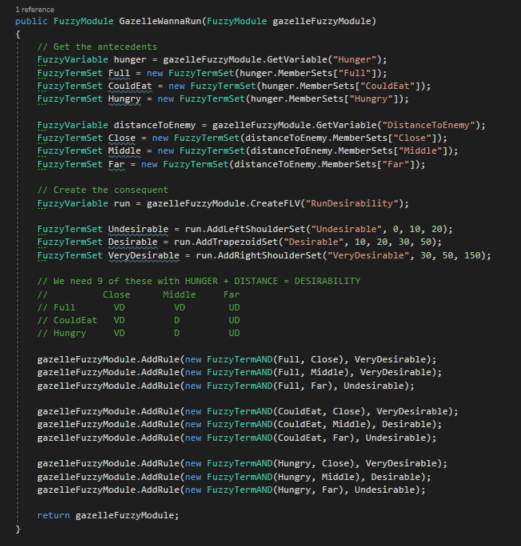
\includegraphics[width=40em]{FuzzyWannaRun.PNG}
    \end{center}
    \caption{Fuzzy wanna run consequence + ruleset}
    \label{fig:FuzzyWannaRun}
\end{figure}
Everything is exactly the same as the above, but with different values and a different ruleset.
Pretty neat and easy, right?
\newpage
\subsection{Class diagram}
\begin{figure}[ht]
    \begin{center}
        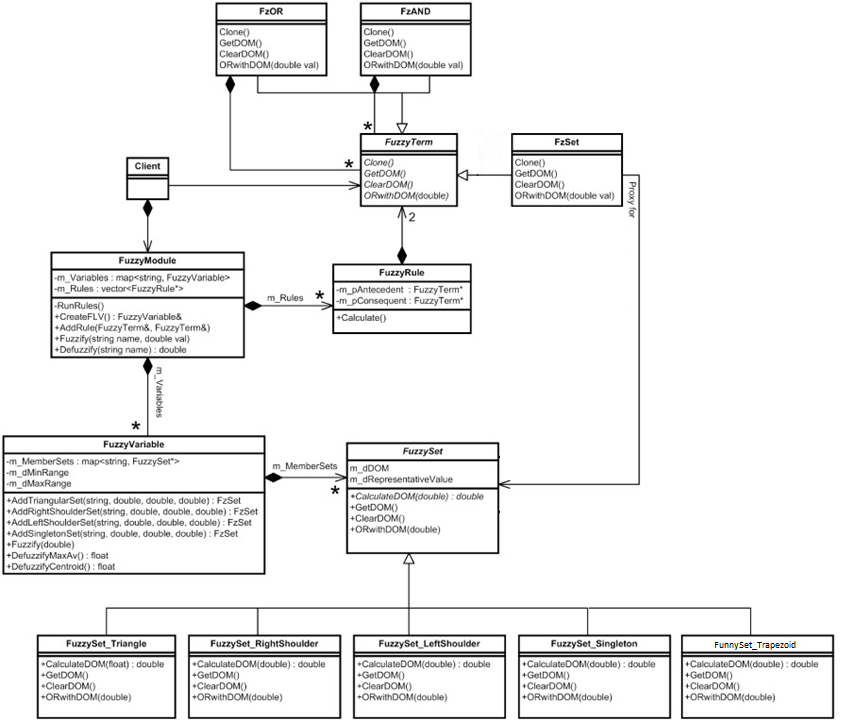
\includegraphics[width=35em]{FuzzyClassDiagram.png}
    \end{center}
    \begin{center}
    \caption{Fuzzy logic class diagram}
    \\Note: This is imported and edited from the following book \cite{pgaie} %TODO: Should be fixed so reference works.
    \end{center}
    \label{fig:FuzzyClassDiagram}
\end{figure}
\newpage
\newpage
%-----------------------------------------------------------------------------------------
    
    \newpage
    %-----------------------------------------------------------------------------------------
    \section{Conclusion}\label{sec:conclusion}
    \subsection[Reflection on the end result]{Reflecion}\label{subsec:reflection}
Looking back at this project I think we did a pretty good job.
Since it was a school exercise we wanted to get it done really fast, and sometimes the development lacked of some testing.
Yet, we tested it good enough to pass working parts of the program to eachother.
So, actually, the not testing wasn't really in our way!
It mainly left some insecurities and we had to hope for the code to work.

Then we wanted to implement everything on the best, neatest possible way and I think that was in our way sometimes.
This way we lost a lot of time thinking things through that actually were finished already.

In the beginning we did a lot of paired programming and I think this cost a lot of time as well.
Mostly since you simply don't have the producing code of two programmers, but of only one.

Looking at these point, you may notice that there was a severe lack of time.
We actually spent a lot of hours on this project, but it was really hard work to get it done in time.

\subsection[Improvements of our project]{Improvements}\label{subsec:improvements}
There are some big improvements that can be done to our game.
This is mainly aimed at the looks of the game, the use of sprites and the behaviours of the animals.

Currently we only used images and not really sprites to represent our entities, this could be a lot better if we just used sprites!
Once again, this was mainly because the lack of time we had.

Then the behaviour of the animals.
With this I mean that we had a limit to how many fuzzy modules / sets we could implement.
The currently implemented fuzzy logic only handles if a gazelle wants to eat or to run from a lion.
The lion can't even decide if it goes after a gazelle yet!
That is a big bummer, because it would be a lot more interactive if this did work.

We also didn't take into account that entities wont flee from another entity if there is an obstacle inbetween.
Right now, we just run from the other entity no matter what.
This would be a pretty easy, but quite essential modification.
Mostly since the gazelle would actually hide behind something and this would look pretty realistic.

The last big improvement I can think of, is some better implementation of the FuzzyLogic into the GoalManager.
Right now we just created a static FuzzyManager to get all configurations for the FuzzyLogic.
We could've implemented this inside the GoalManager much more beautiful (for \textbf{instance} (hehe..) a non-static class).

    
    \newpage
    %-----------------------------------------------------------------------------------------

    \addcontentsline{toc}{section}{References}
    \begin{thebibliography}{9}
        \bibitem{pgaie}
        Mat Buckland (2004).
        \textit{Programming Game AI by Example}.
        Wordware, 2004

        \bibitem{aapc}
        Lluis Alseda.
        \textit{A* Algorithm pseudocode}
        \\\textit{\url{http://mat.uab.cat/~alseda/MasterOpt/AStar-Algorithm.pdf}}
        \\\textit{Accessed: 2018-04-01}
    \end{thebibliography}
\end{document}